%! TEX root = main.tex

\section{Solución}


Se diseña y desarrolla un Juego Serio para dispositivos móviles llamado
\textit{eTesai}, el cual ofrece a los estudiantes de enfermería un medio para
realizar procedimientos de enfermería y cuyo objetivo es servir como herramienta
de apoyo al aprendizaje. La solución propuesta permite evaluar a los juegos
serios en los aspectos de diseño, implementación y evaluación.

Los procedimientos simulados son seleccionados en conjunto con los profesionales
del área de enfermería del \gls{iab} y son, la venopunción
y la evaluación del paciente utilizando la escala de \textit{Glasgow}. 

\subsection{Arquitectura}

En la figura~\ref{fig:full_architecture} se observa la arquitectura general de la 
solución.

\begin{figure}[H]
\centering
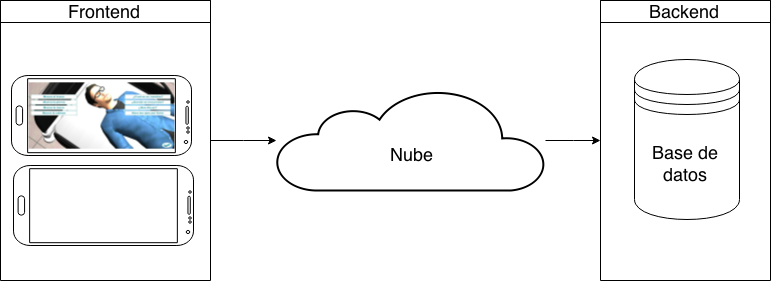
\includegraphics[scale=0.29]{images/full.png}
\caption{Esquema general de componentes de la solución.}
\label{fig:full_architecture}
\end{figure}

La solución se compone de un \textit{front-end}\footnote{El \textit{front-end}
    es la parte de la solución que interactúa con el usuario. Se encarga de
    realizar una simulación, de interpretar las acciones del usuario y evaluar
    el rendimiento del usuario.} que consiste en una aplicación \textit{Android}, la cual
es utilizada por los estudiantes de enfermería. Los registros de uso del
\textit{front-end} son almacenados bajo demanda en un servidor
\textit{back-end}\footnote{El \textit{back-end} es la parte de la solución que
    se encarga de almacenar la información de los usuarios y sus acciones dentro
    del \textit{front-end}.}, el cual se encarga de asociar los registros con
los alumnos y almacenarlos de manera persistente.

\subsection{Tecnologías utilizadas}

El motor de videojuegos utilizado para el desarrollo del \textit{front-end} es
\textit{Unity3D}, en su versión gratuita. \textit{Unity3D} es desarrollado por
\textit{Unity Technologies} y posee un motor de \textit{renderizado}, un flujo
de trabajo para la creación de contenido interactivo, y permite mezclar
contenido 3D, 2D, sonidos y animaciones en un entorno de desarrollo integrado.
\textit{Unity3D} permite desarrollar aplicaciones para múltiples sistemas
operativos, como \textit{Android, iOs, Windows Phone}, entre
otros\cite{unity3d}. El código fuente del \textit{front-end} es desarrollado con
\textit{MonoDevelop}.

% Agregar referencias
El \textit{back-end} es desarrollado utilizando \textit{Java EE 7}, servicios web
\textit{REST}, y \textit{Eclipse} como entorno de desarrollo integrado. 

\subsection{Front-end}

El \textit{front-end} consiste en una aplicación \textit{Android}, con un flujo que se observa en la
figura~\ref{fig:flujo_frontend}, la misma se inicia en la escena \emph{Inicio},
que permite al usuario seleccionar varias opciones y navegar a las demás
escenas.

\begin{figure}
\centering
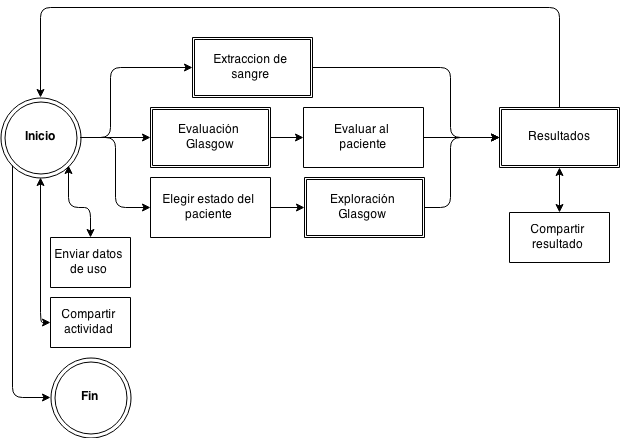
\includegraphics[width=8.5cm]{../solucion/images/grafo_escenas.png}
\caption{Flujo de pantallas de la solución}
\label{fig:flujo_frontend}
\end{figure}

La simulación posee dos mecanismos para interactuar con el punto de vista del
usuario, \textit{a)} alejar o acercar la cámara, y, \textit{b)} mover la cámara
alrededor del paciente.

Las acciones realizadas por los usuarios, así como el resultado de sus acciones,
son registradas en el dispositivo del usuario, y luego son enviadas al
\textit{back-end} para su persistencia.

\subsection{Back-end}

El servidor \textit{back-end} almacena la información del usuario, se encarga
de recibir y asociar los datos almacenados por el \textit{front-end} en una
base datos para su posterior análisis.


Almacena información detallada acerca de las acciones del usuario,
las condiciones de estas acciones y el contexto en el cual fueron ejecutadas.
La información almacenada permite reproducir las sesiones de juego
de los usuarios. Esta información es útil para analizar los puntos débiles y
fuertes, tanto de los usuarios como de la solución.

\subsection{Selección de procedimientos}

La selección de los procedimientos que formarán parte de la solución se realiza
conjuntamente con los profesores del \Gls{iab} y son los siguientes:

\begin{itemize}
\item \textbf{Venopunción:} es utilizado frecuentemente para extraer muestras de
    sangre. Fue seleccionado debido a que: posee pasos bien definidos que deben
    ser seguidos por el profesional de enfermería, la complejidad del
    procedimiento no es muy alta y sus pasos son susceptibles de equivocaciones.
    El procedimiento formal, según los profesores del \gls{iab}
    y~\cite{oms:extraccion}, cuenta con $22$ pasos.
\item \textbf{Valoración de la escala de Glasgow:} es utilizada como una
    herramienta de valoración objetiva del estado de conciencia de pacientes en
    estado crítico. Consiste en la evaluación de la respuesta motora, verbal y
    ocular del paciente\cite{protocolo}. Fue seleccionado debido a que: permite
    la exploración del entorno pues hay diferentes formas de evaluar cada estado
    del paciente, rara vez es realizado pues las condiciones necesarias para que
    un paciente requiera que se le realice este procedimiento son críticas, la
    cantidad de reacciones que evalúa el procedimiento es muy alta y no es un
    procedimiento complejo. 
\end{itemize}

\subsection{Alcance}

Realizar una simulación de todos los aspectos que están presentes en un
procedimiento de enfermería es un proceso complejo. Cuando existe una gran
cantidad de detalles, los usuarios tienden a centrase en estos detalles y no en
los factores pedagógicos\cite{videojuegos:gonzaleztardon}, por esto, uno de los
objetivos de la solución es la presentación de situaciones simplificadas que
permitan construir conocimiento.

Las limitaciones técnicas\footnote{Las limitaciones técnicas se relacionan con
    la dificultad para simular un determinado paso, teniendo en cuenta
    consideraciones de \textit{hardware, software} y tiempo.}, la importancia de
la representación\footnote{La importancia de representación se refiere a que tan útil es
    un determinado paso para los objetivos pedagógicos.} y la facilidad de
realización\footnote{La facilidad de realización en la vida real
    se refiera a que tan fácil es realizar el paso en la vida real.} son los
factores utilizados para acotar el alcance de la simulación.

Algunas acciones requieren un esfuerzo significativo para ser simuladas y deben
formar parte del procedimiento. El nivel de detalle simulado para estas acciones
no es importante, por ello se formulan las siguientes hipótesis que permiten
guiar la simulación de los mismos:


\begin{enumerate}[\bfseries H1.:]
%\begin{enumerate}[label=\bfseries H\arabic*:]

\item \textbf{Interacción a través de la voz}: para enviar una petición o
    informarle sobre algo al paciente, no es necesario utilizar reconocimiento
    del habla, sino más bien detectar que el usuario ha hablado y listar las posibles
    acciones que se puedan realizar. Los comandos de voz hacen más interactiva a
    la \gls{gui}.
    
\item \textbf{Extracción de elementos}: para realizar la acción de extraer un
    elemento utilizado en el paciente, se considera que realizarlo de una sola
    manera para todos los elementos disponibles en la solución aporta una
    interfaz más intuitiva.

\item \textbf{Bioseguridad}: la bioseguridad\footnote{La bioseguridad es la
        aplicación de conocimientos, técnicas y equipamientos para prevenir a
        personas, laboratorios, áreas hospitalarias y medio ambiente de
        exposición a agentes potencialmente infecciosos o considerados de riesgo
        biológico\cite{world2005manual}.} es un área amplia y transversal a
    todos los procedimientos de enfermería, por lo que se considera complejo
    simular cada acción. Es suficiente que el usuario sepa en que momento
    realizar cada una de las acciones. Realizar la simulación de todos los
    procedimientos de bioseguridad escapa al alcance del trabajo.

\item \textbf{Representación iconográfica}: para representar el estado de los
    objetos es suficiente mostrar una imagen representativa. Ciertos estados son
    complejos de simular (como la esterilización de las manos), realizar una
    simulación de los estados de los objetos es complejo y requiere un nivel de
    detalle que desviará al usuario de los objetivos pedagógicos.
    
\item \textbf{Motivación}: indicadores de rendimiento, como un puntaje al final
    de cada procedimiento, y el tiempo total dentro del procedimiento, impactan
    positivamente en el involucramiento del usuario. La interacción social es
    otro factor que incrementa el nivel de compromiso del usuario.

\item \textbf{Retroalimentación limitada}: la ausencia de signos visuales que
    indiquen las acciones que debe realizar el usuario durante la experiencia,
    permite al usuario probar sus conocimientos, y le impide avanzar en
    el procedimiento utilizando una técnica de \emph{prueba y error}.

\item \textbf{Movilidad}: el uso de la solución en los dispositivos móviles de
    los usuarios permite más oportunidades de poner a prueba los conocimientos
    con respecto a alternativas tradicionales.

\end{enumerate}

\subsection{Escenas}

La solución presenta procedimientos de enfermería en forma de escenas simuladas.
%Los procedimientos son seleccionados en conjunto con profesionales del área de
%enfermería del \gls{iab}. 

El procedimiento de venopunción, es representada dentro de la solución en la
escena \emph{Venopunción}. El procedimiento de evaluación de un paciente
utilizando la escala de \textit{Glasgow}, es representado en la escena
\emph{Glasgow}.

\subsection{Venopunción}

En la figura~\ref{fig:hemocultivo_principal} se observa el inicio de la escena,
el objetivo principal de este procedimiento es extraer muestras de la sangre del
paciente para su análisis en un laboratorio.

\begin{figure}[H]
\centering 
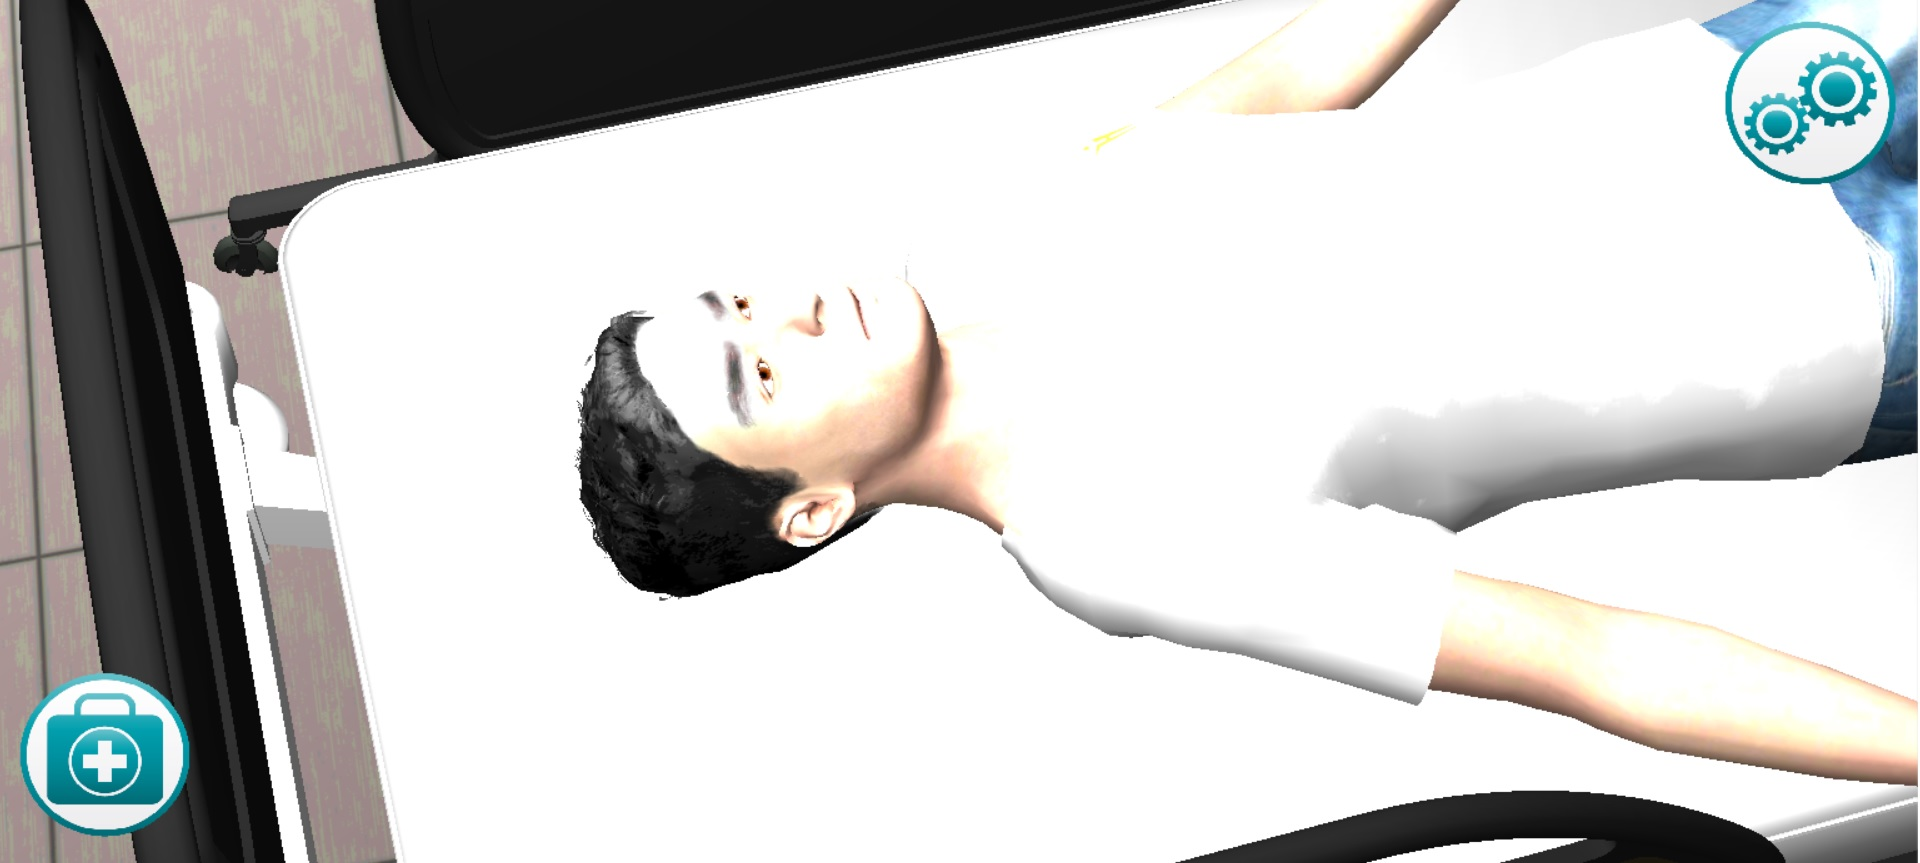
\includegraphics[width=8cm]{../solucion/images/hemocultivo_principal.jpg}
\caption{Pantalla principal de la escena \emph{Venopunción}.}
\label{fig:hemocultivo_principal}
\end{figure}

Durante la escena el usuario interactúa con varios objetos, en la
figura~\ref{fig:hemocultivo_jeringa_zoom} se observa la jeringa en el brazo del
paciente, con flechas ilustrativas que muestran como mover los dedos para
realizar la extracción de la sangre.

\begin{figure}[H]
\centering 
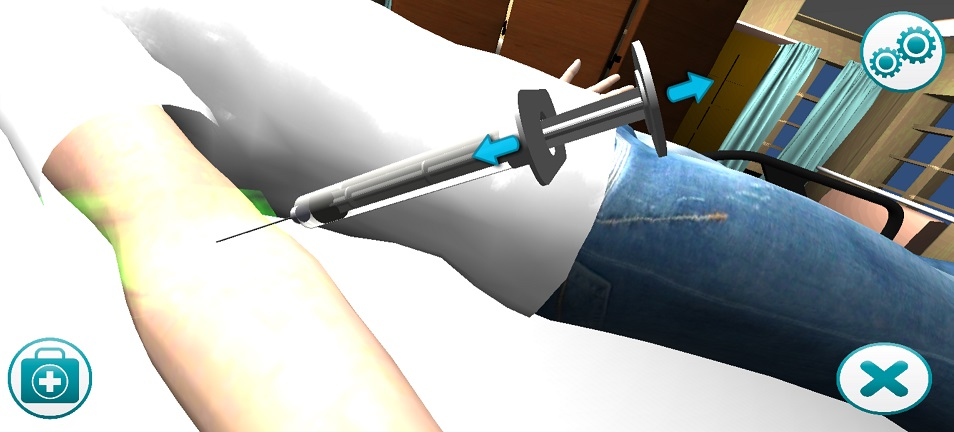
\includegraphics[width=8cm]{../solucion/images/hemocultivo_jeringa_ampliada.jpg}
\caption{Vista de la jeringa ampliada, facilitando la extracción de sangre.}
\label{fig:hemocultivo_jeringa_zoom}
\end{figure}

En la figura~\ref{fig:hemocultivo_gui} se observa la interfaz gráfica, con
opciones de bioseguridad y de utilización de elementos.

\begin{figure}
\centering
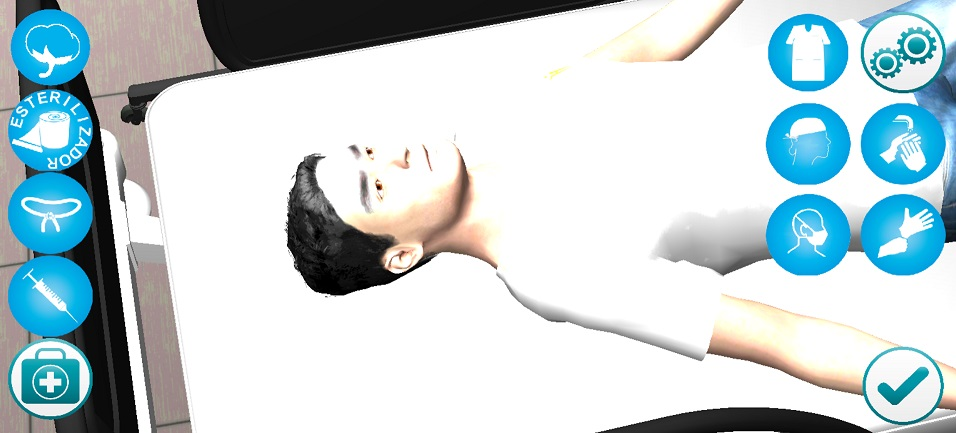
\includegraphics[width=8cm]{../solucion/images/hemocultivo_gui.jpg}
\caption{Interfaz gráfica de la escena \emph{Venopunción}}
\label{fig:hemocultivo_gui}
\end{figure}

La evaluación del desempeño del alumno durante la partida se utiliza un
motor de \gls{eca}\cite{bailey2004event,behrends2006combining}, este motor
permite reaccionar ante las acciones del usuario y verificar el cumplimiento de
los pasos del procedimiento. 

\begin{figure}
\centering 
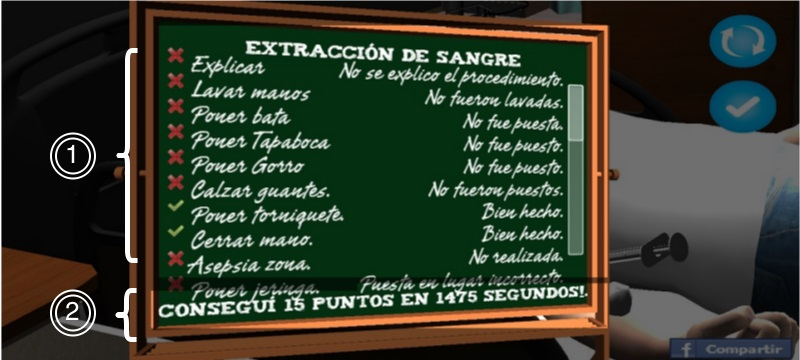
\includegraphics[width=8cm]{../solucion/images/hemocultivo_retroalimentacion.jpg}
\caption{Retroalimentación y puntuación final de la escena \emph{Venopunción}.}
\label{fig:hemocultivo_retroalimentacion}
\end{figure}

En la parte $1$ de la figura~\ref{fig:hemocultivo_retroalimentacion}, se observa
la información que la solución provee al usuario acerca de su rendimiento. Esta
información le indica los pasos que realizó de manera correcta o incorrecta y
las razones por las cuales tuvo ese desempeño.

Cada regla tiene asociado un peso, de acuerdo a la dificultad de realizar el
paso, este peso es utilizado al final de la partida para dar una puntuación al
usuario como se muestra en el punto $2$ de la
figura~\ref{fig:hemocultivo_retroalimentacion}. Junto al puntaje final también
se muestra el tiempo que le tomó al usuario completar el procedimiento.

\subsection{Glasgow}


%Permite al usuario explorar el entorno, es un procedimiento que requiere un
%%nivel alto de pericia, y solo algunos alumnos tienen la posibilidad de
%realizarlo durante las prácticas de campo debido a que requiere pacientes en
%estado crítico. 
El objetivo principal de esta escena es diagnosticar el estado de conciencia de
un paciente en estado crítico, utilizando la escala de \textit{Glasgow}. 

La interfaz principal se observa en la figura~\ref{fig:glasgow_principal}, se
observa al paciente a diagnosticar. Esta escena tiene dos versiones. La primera
versión, denominada \emph{Evaluación}, se inicia con un paciente en un estado
aleatorio, la tarea del alumno es diagnosticar el estado del paciente. En la
segunda versión, denominada \emph{Exploración}, el usuario elige el estado
inicial del paciente, lo que le permite observar como reacciona un paciente con
un diagnóstico dado.

\begin{figure}[H]
\centering
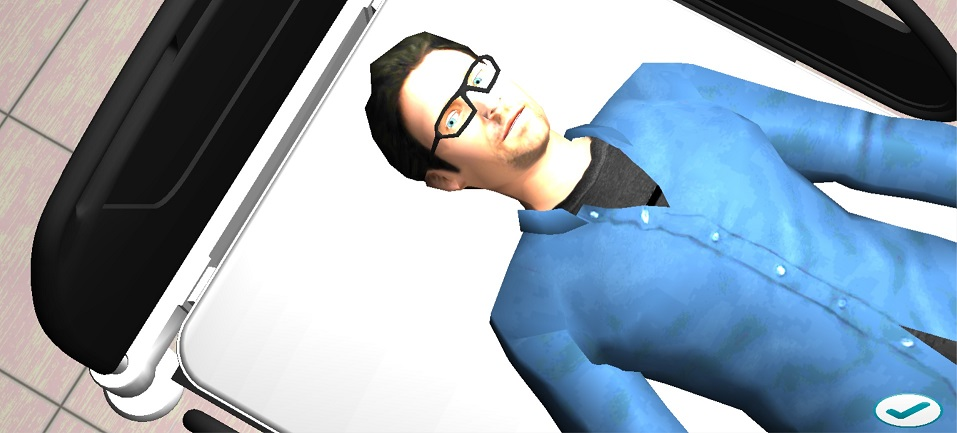
\includegraphics[width=8cm]{../solucion/images/glasgow_principal.jpg}
\caption{Interfaz de la escena de \emph{Valoración de la escala de Glasgow.}}
\label{fig:glasgow_principal}
\end{figure}



El protocolo indica que el enfermero debe valorar tres aspectos del paciente,
la visión (del $1$ al $4$), la audición (del $1$ al $5$) y la capacidad motora
(del $1$ al $6$)\cite{protocolo}. Realizada la valoración del
paciente, el enfermero debe sumar los puntajes obtenidos, y así realizar un
diagnóstico, de $13$ a $15$ el daño es leve, de $9$ a $12$ el daño es moderado y
de $3$ a $8$ el daño es severo\cite{helmick2007mild}.


\begin{figure}[H]
\centering
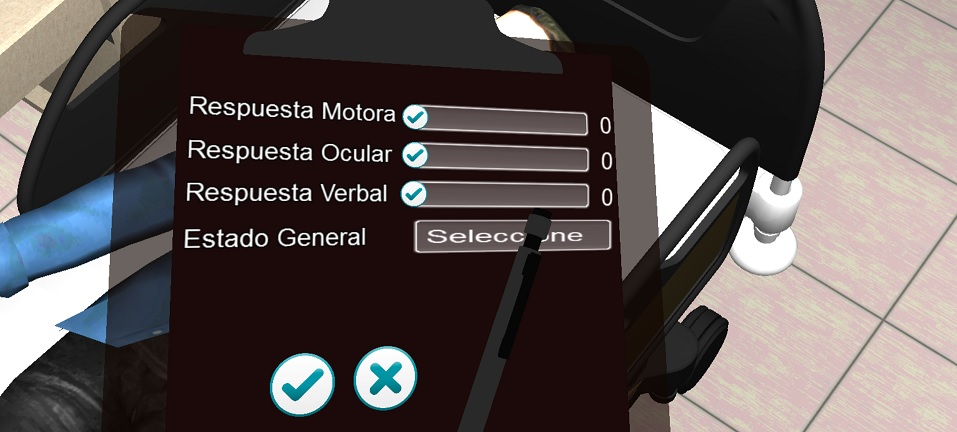
\includegraphics[width=7.5cm]{../solucion/images/glasgow_diagnostico.jpg}
\caption{Vista de la \emph{Pantalla de diagnóstico}.}
\label{fig:glasgow_gui_resultados}
\end{figure}

El diagnostico del usuario es contrastado con el estado real del paciente, para
mostrar el resultado de la escena, en el punto $1$ de la
figura~\ref{fig:glasgow_resultado} se observa la retroalimentación dada al
usuario.

Para el cálculo del puntaje final, por cada respuesta dada en la \emph{Pantalla
    de diagnóstico} se asigna una puntuación de acuerdo a que tan cerca estuvo
el usuario de la respuesta correcta. Se suman estos valores y se calcula el
porcentaje de acierto. El puntaje final junto al tiempo que tardó el usuario
realizando el procedimiento son presentados como se observa en el punto $2$ de
la figura~\ref{fig:glasgow_resultado}.

\begin{figure}[H]
\centering
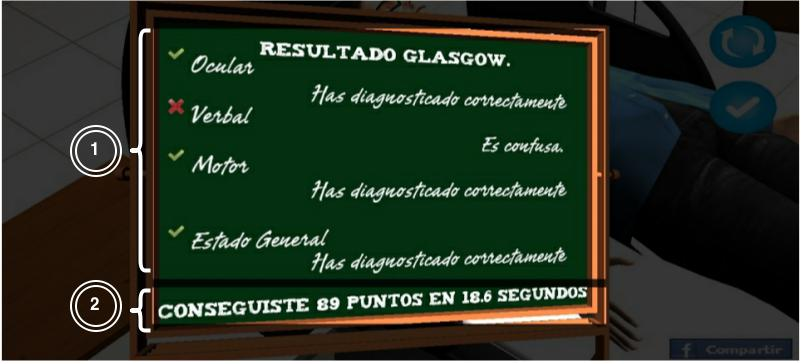
\includegraphics[width=7.5cm]{../solucion/images/glasgow_resultado.jpg}
\caption{Retroalimentación y puntuación final de la escena \emph{Glasgow}.}
\label{fig:glasgow_resultado}
\end{figure}
